\documentclass[12pt,a4paper,headsepline]{scrreprt}

\usepackage{ucs}
\usepackage[utf8x]{inputenc}
\usepackage[T1]{fontenc}
\usepackage[ngerman]{babel}
\usepackage{blindtext}
\usepackage{scrlayer-scrpage}
\usepackage{graphicx}
% \usepackage{footnote}
\usepackage{amsfonts}
\usepackage{amsmath}
\usepackage[onehalfspacing]{setspace}
\usepackage[
	left=2.6cm,
	right=2.8cm,
	top=2.5cm,
	bottom=2.5cm
			]{geometry}
%\newgeometry{
%  left=3cm,
%  right=3cm,
%  top=2.5cm,
%  bottom=2.5cm,
%  bindingoffset=0mm
%}
% Listoffigures, Listoftables, Listofindex werden in Toc angezeigt
% \usepackage{tocbibind}

% Moderne Schriftart wird verwendet
\usepackage{lmodern}
\usepackage{textcomp} %bestimmte sonderzeichen
\newcommand{\eur}[1]{\mbox{#1\,\texteuro}\xspace}
% Tabellen ---------------------------------------------------------------------
\PassOptionsToPackage{table}{xcolor}
\usepackage{tabularx}
% für lange Tabellen
\usepackage{longtable}
\usepackage{array}
\usepackage{ragged2e}

% pdfs einbinden
\usepackage{pdfpages}

\usepackage{lscape}
\newcolumntype{w}[1]{>{\raggedleft\hspace{0pt}}p{#1}}
\usepackage{xcolor}
\usepackage{url}
% Tabellen-, Equation- und Figurenummerierung ist nicht Chapter gebunden
\usepackage{chngcntr}
\counterwithout{table}{chapter}
\counterwithout{equation}{chapter}
\counterwithout{figure}{chapter}
% Tabellen werden nicht nach Chapter nummeriert
\renewcommand{\thetable}{\arabic{table}}

% Abstand zwischen Nummerierung und Überschrift definieren
% > Schön wäre hier die dynamische Berechnung des Abstandes in Abhängigkeit
% > der Verschachtelungstiefe des Inhaltsverzeichnisses
\newcommand{\headingSpace}{1.5cm}
% Für die Einrückung wird das Paket tocloft benötigt
\usepackage[titles]{tocloft}
%\cftsetindents{chapter}{0.0cm}{\headingSpace}
%\cftsetindents{section}{0.0cm}{\headingSpace}
%\cftsetindents{subsection}{0.0cm}{\headingSpace}
%\cftsetindents{subsubsection}{0.0cm}{\headingSpace}
%\cftsetindents{figure}{0.0cm}{\headingSpace}
%\cftsetindents{table}{0.0cm}{\headingSpace}

\setlength{\parindent}{0em}
\usepackage{makeidx}
\usepackage{varioref}
\usepackage{hyperref}
\hypersetup{%
  linktocpage 	= true,
  colorlinks  	= true,
  linkcolor   	= blue,
}

% Tabellenfärbung:
\definecolor{heading}{RGB}{100,165,245}
%\definecolor{heading}{rgb}{0.64,0.78,0.86}
\definecolor{odd}{rgb}{0.9,0.9,0.9}

% fügt Tabellen aus einer TEX-Datei ein
\newcommand{\tabelle}[3]{
\begin{table}[htbp]
\centering
\singlespacing
\input{#3}
\caption{#1}
\label{#2}
\end{table}}

\newcommand{\Anhang}[1]{\appendixname{}~unter~\ref{#1}: \nameref{#1}}
\newcommand{\tab}[1]{Tabelle~\ref{#1}~\nameref{#1}}
\newcommand{\sectionref}[1]{\ref{#1}~\nameref{#1}}
\newcommand{\bildref}[1]{\ref{#1}~\nameref{#1}}
\renewcommand{\thetable}{\arabic{table}}

\automark{chapter}
\automark*{section}
\clearpairofpagestyles
%\ihead{\headmark}
%\ihead{\footnotesize Migration und Modifikation der autoritativen DNS-Infrastruktur \\mit der Implementierung von DNSSEC}
%\ohead{\includegraphics[scale=0.047]{Bilder/logo_interchalet.png} }
\ifoot{Viktor Gange - Mt. 4924109}
\ofoot{\pagemark}
\renewcommand*\chapterpagestyle{scrheadings} 	% Die erste Chapter Seite bekommt auf die
												% Weise auch einen Header

\begin{document}
\pagenumbering{arabic}


% Inhalt
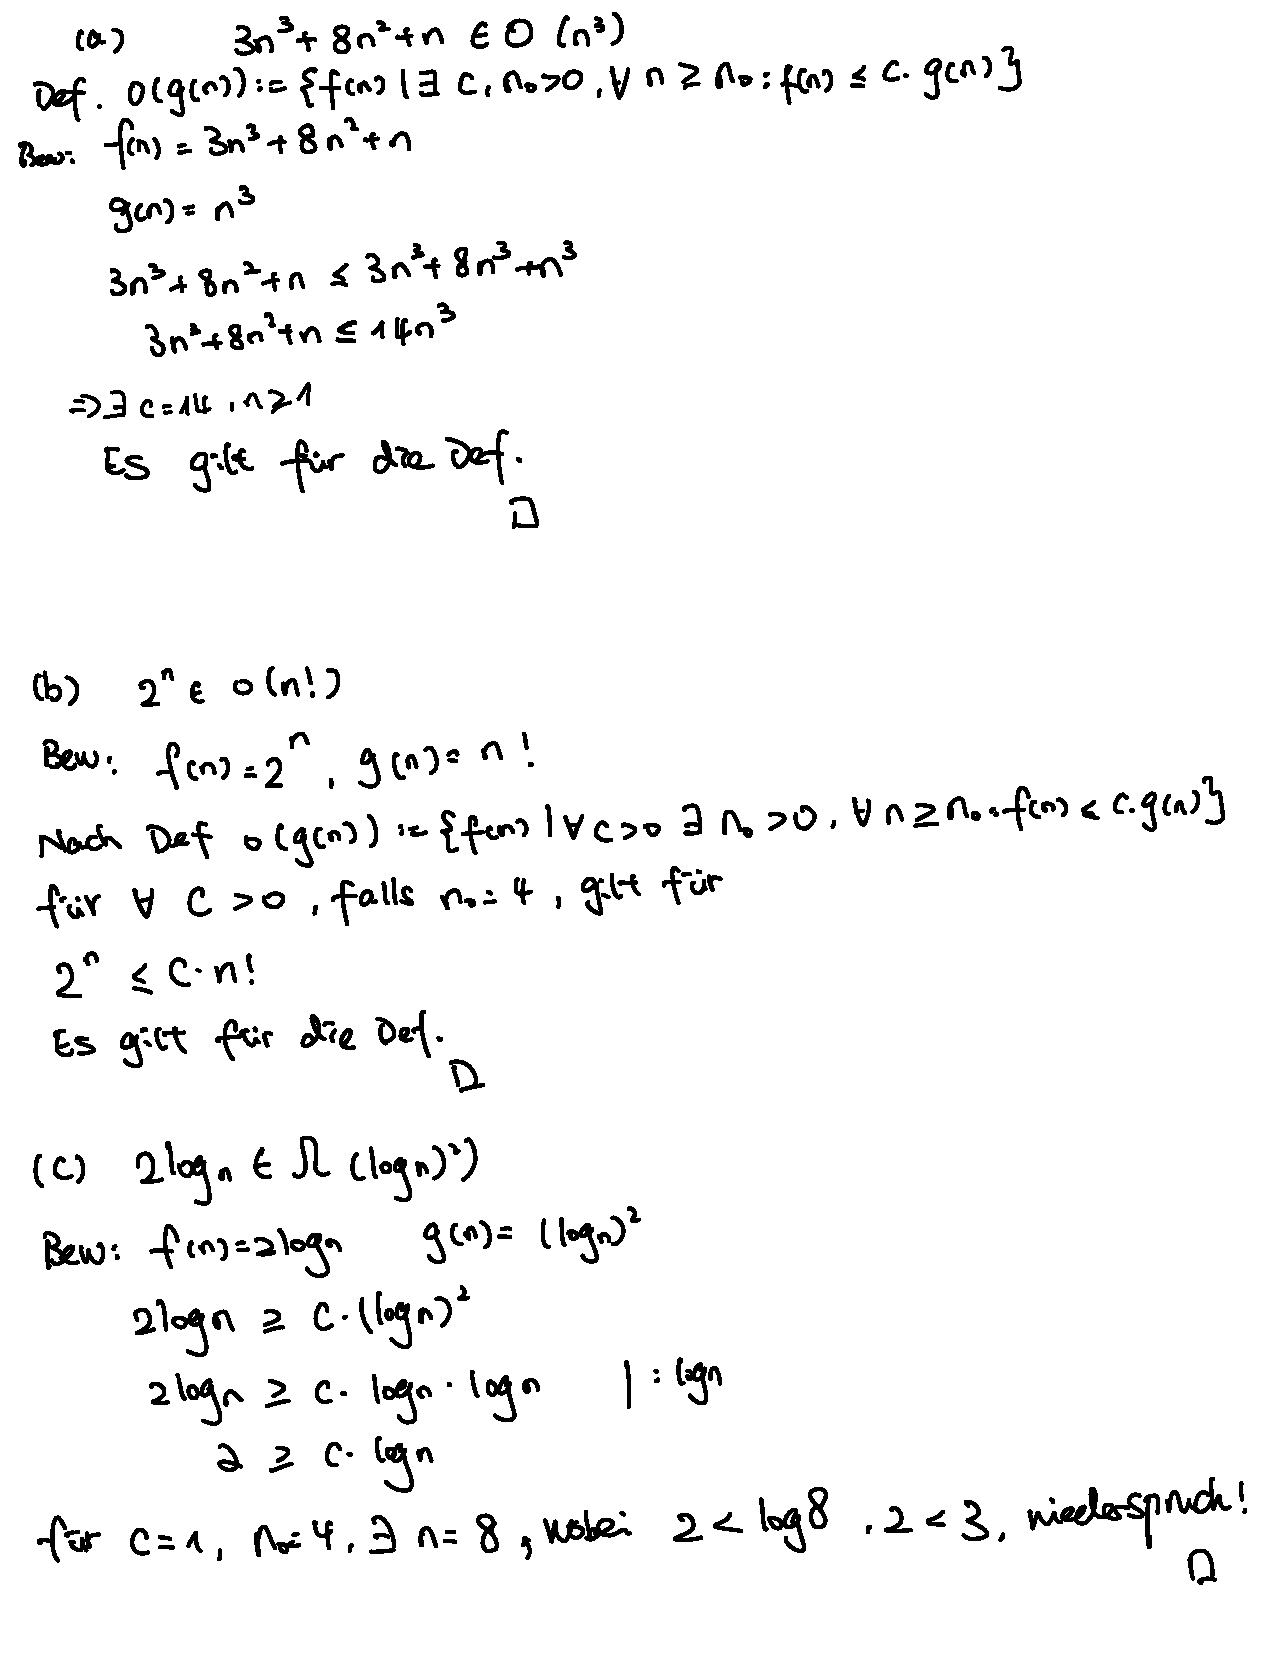
\includepdf[scale=.8,pagecommand=\section*{Aufgabe 1},page={1}]{Blatt02_Aufgabe1.pdf}
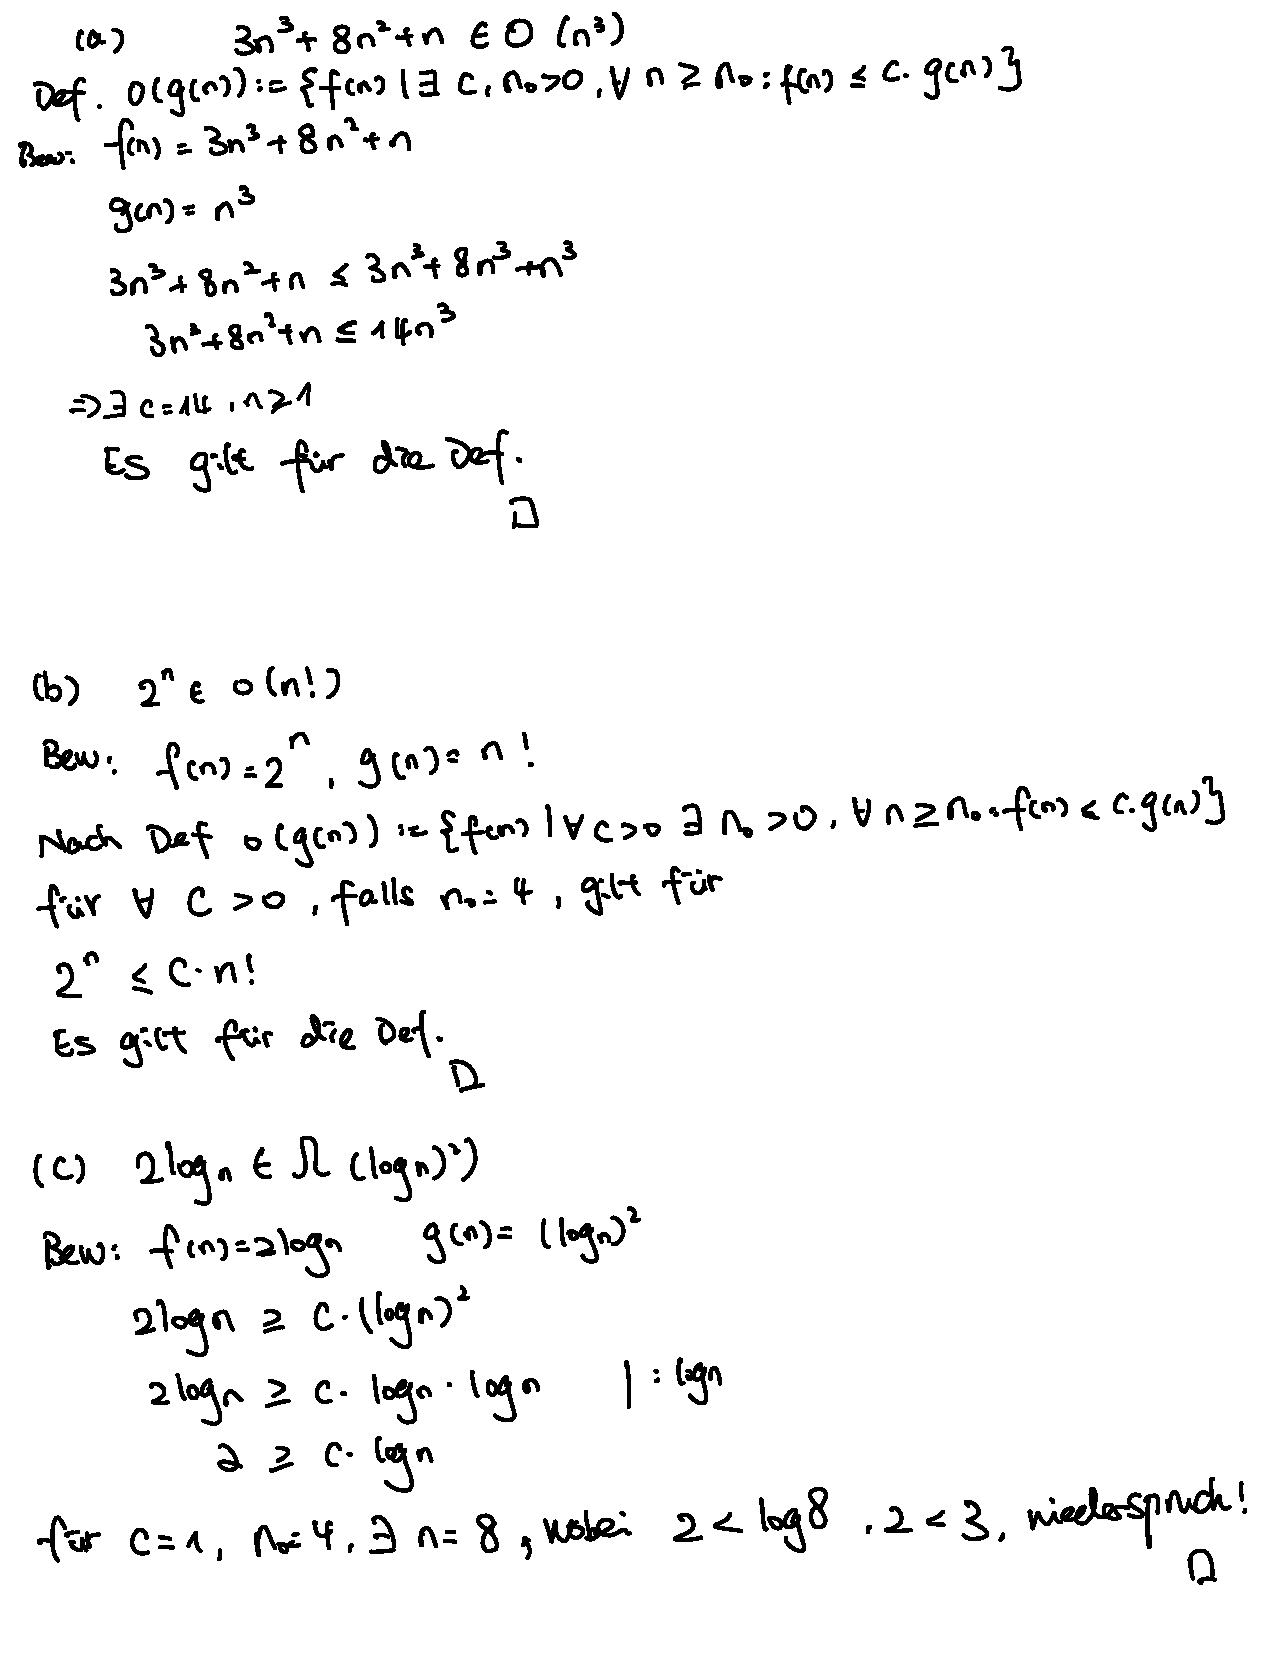
\includepdf[scale=.8,page={2}]{Blatt02_Aufgabe1.pdf}

\section*{Aufgabe 2}
$2^{n^2}~>~n^n~>~(n+1)!~=~n!~>~(2^n)^2~>~3^n~>~2^n~>~n^{100}~>~10^{100}n~>~\\n\log n~>~\sqrt{n}~>~(\log n)^2~>~\log n^3~=~\log n~=~\log \sqrt{n}~>~\sqrt{\log n}$

\section*{Aufgabe 3}
\textbf{a)}\\
In der Vorlesung wurden diese vier Algorithmen gezeigt:\\
Selectionsort, Insertionsort, Mergesort und Quicksort.\\
Davon sind jedoch nur Insertion sort und Mergesort stabil.\\

\textbf{Beispiel für Selectionsort:}\\
Die Zahlen in Klammern sind die Startindices\\

unsorted array $=[2,1,4(2),6,4(4),3]$\\

Wenn man jetzt mit dem Selectionsort aus der Vorlesung sortiert, dann bekommt man folgendes Array:\\
sorted array $=[1,2,3,4(4),4(2),6]$\\

Die einzelnen Schritte sind:\\
$2\rightarrow1,~~ 2\rightarrow2,~~ 4(2)\rightarrow3,~~ 6\rightarrow4(4),~~ 6\rightarrow4(2),~~ 6\rightarrow6$\\

Wie man sieht sind die beiden 4 in der falschen Reihenfolge, das bedeutet, dass Selectionsort instabil ist.\\

\textbf{b)}\\
\textbf{Selectionsort:}\\
Wir würden beim Aufruf von Selectionsort am Anfang ein weiteres Array mit dem Startindex der Einzelnen Komponente befüllen.
Also zum Beispiel:\\
$[0,1,2,3]$ für eine liste mit 4 Elementen.\\

Bei jedem Tausch von Elementen im Hauptarray, sollte auch im Indexarray die Indices getauscht werden, also zum Beispiel:\\
Hauptarray: $[5,3,1]$\\
Indexarray: $[0,1,2]$\\
Tausch von 5 und 1 im Hauptarray:\\
$[5,3,1] \rightarrow [1,3,5]$\\
Also wird auch im Indexarray getauscht:\\
$[0,1,2] \rightarrow [2,1,0]$\\

Ein letzten Schritt den wir machen müssen, ist eine weitere If-bedingung einbauen, die bei gleichen Elementen die Indices im Indexarray überprüft.\\

Damit wissen wir also welches Element, wenn diese gleich sind(zum Beispiel 4 und 4), im Startarray den kleineren Index hatte, und können somit Stabil sortieren.\\



\end{document}
